\documentclass[12pt,aspectratio=169]{beamer}

%
\usepackage{algorithm,algorithmic}
%
%\usepackage[utf8]{inputenc}
%\usepackage{booktabs}
%\usepackage[opacity=0.1]{pdfcomment} % set to 0 to make annotation icons invisible
%\usepackage{pdfpc}
%\usepackage{arev}
%\usepackage{multicol}
%
%\usepackage{xcolor, color, colortbl}
%\definecolor{dkgreen}{rgb}{0,0.5,0}
%\definecolor{dkred}{rgb}{0.8,0,0}
%\definecolor{dkblue}{rgb}{0,0,0.5}
%\definecolor{gray}{rgb}{0.5,0.5,0.5}
%\definecolor{mauve}{rgb}{0.58,0,0.82}
%\definecolor{hilight}{RGB}{122,86,0}
%
%\definecolor{LRed}{rgb}{1,.8,.8}
%\definecolor{MRed}{rgb}{1,.6,.6}
%\definecolor{HRed}{rgb}{1,.2,.2}
%
%%Information to be included in the title page:
%
%\tikzset{
%        ->,  % makes the edges directed
%        >=stealth', % makes the arrow heads boldnode 
%        distance=3cm, % specifies the minimum distance between two nodes. Change if necessary.
%        every state/.style={thick, fill=gray!10}, % sets the properties for each ’state’ node
%        initial text=$ $, % sets the text that appears on the start arrow
%}
%
%\def\firstcircle{(90:1.75cm) circle (2cm)}
%\def\secondcircle{(210:1.75cm) circle (2cm)}
%\def\thirdcircle{(330:1.75cm) circle (2cm)}
%
%\usepackage{tikz}
%\usetikzlibrary{arrows.meta,
%                calc, chains,
%                quotes,
%                positioning,
%                shapes.geometric}
%
%
%\def\scalefact{0.85}
%\newcommand{\cev}[1]{\reflectbox{\ensuremath{\vec{\reflectbox{\ensuremath{#1}}}}}}
%\newcommand{\evalat}[2]{\left.#1\right\vert_{#2}}
%
%\newcommand{\znode}[5][black]{\path (#3,#4) node(#2) [circle,draw,color=#1] {#5};}
%\newcommand{\zunedge}[6][black]{%
%\begin{scope}
%	\path (#2,#3) node(this) [inner sep=0pt,triangle,draw,color=#1] {#4};
%	\draw[->,color=#1] (#5) -- (this.west);
%	\draw[->,color=#1] (this.east) -- (#6);
%\end{scope}}
%\newcommand{\zbiedge}[7][black]{%
%\begin{scope}
%	\path (#2,#3) node(this) [inner sep=0pt,triangle,draw,color=#1] {#4};
%	\draw[->,color=#1] (#5) -- (this);
%	\draw[->,color=#1] (#6) -- (this);
%	\draw[->,color=#1] (this.east) -- (#7);
%\end{scope}}
%\newcommand{\zedge}[5][black]{\path (#3,#4) node(#2) [inner sep=0pt,triangle,draw,color=#1] {#5};}
%
%\definecolor{blue(pigment)}{rgb}{0.2, 0.2, 0.6}
%\definecolor{burgundy}{rgb}{0.5, 0.0, 0.13}
%
%
%\usepackage{listings}
%%% \usetheme{Goettingen}
%\usefonttheme{serif}
%\usepackage{times}
%\setbeamertemplate{navigation symbols}{}
%
%\title{Perceptron}
% 
% 
%%\author[Mehrdad Maleki] % (optional, for multiple authors)
%%{Mehrdad Maleki, Barak A. Pearlmutter\footnote{ Institute & Department of Computer Science
%%Maynooth University, Co. Kildare, Ireland}, Jeffrey Mark Siskind}
% 
%%\institute[NUIM] % (optional)
%%{
%%  Department of Computer Science \\
%%  National University of Ireland Maynooth
% 
%%}


\usepackage[utf8]{inputenc}
%\usepackage[table]{xcolor}
\usepackage{color, colortbl}
\definecolor{LRed}{rgb}{1,.8,.8}
\definecolor{MRed}{rgb}{1,.6,.6}
\definecolor{HRed}{rgb}{1,.2,.2}
\usepackage{tikz}
\definecolor{Gray}{gray}{0.9}
\definecolor{Green}{rgb}{0.3,0.9,0.3}
\definecolor{Red}{rgb}{0.98,0.3,0.3}
\usetikzlibrary{automata, positioning, arrows}
%Information to be included in the title page:

\tikzset{
        ->,  % makes the edges directed
        >=stealth', % makes the arrow heads boldnode 
        distance=3cm, % specifies the minimum distance between two nodes. Change if necessary.
        every state/.style={thick, fill=gray!10}, % sets the properties for each ’state’ node
        initial text=$ $, % sets the text that appears on the start arrow
}

\usepackage{tkz-euclide}


\def\firstcircle{(90:1.75cm) circle (2cm)}
\def\secondcircle{(210:1.75cm) circle (2cm)}
\def\thirdcircle{(330:1.75cm) circle (2cm)}

%\usetheme{Madrid}

\title[Finite Automata] %optional
{Deep Learning}
 
\subtitle{Lecture 1: Linear Algebra}
 
%\author[Maleki] % (optional, for multiple authors)
%{Dr. Mehrdad Maleki}
% 
%\institute[NUIM] % (optional)
%{
%  Department of Computer Science \\
%  National University of Ireland Maynooth
% 
%}
 
\date{February 2020}

\author[]{\textbf{Dr. Mehrdad Maleki}}
 
\date{}
 
%\logo{\includegraphics[height=1.5cm]{lion-logo.png}}

\renewcommand{\Re}{\mathbb{R}}
 
\begin{document}
 
\frame{\titlepage}

\newcommand{\SYSTEM}[2]{\raisebox{-1ex}{\shortstack{#1\\[-0.25ex]\tiny #2}}}
\newcommand{\YES}{\textcolor{dkgreen}{$\ballotcheck$}}
\newcommand{\NOPE}{\textcolor{dkred}{$\ballotx$}}
\newcommand{\MAYBE}{\textcolor{dkblue}{\textbf{?}}}




\begin{frame}
\frametitle{Sets}
\begin{itemize}
\item \textbf{Set} is a collection of objects represented as a unit.
\bigskip \pause
\item A set with no elements is called the \textbf{empty set} and is denoted by $\emptyset$. So $\emptyset=\{\;\}$.\pause
\item Set $A=\{a,b,c\}$ is the same as the set $B=\{b,c,a\}$.
\bigskip \pause
\item There is no duplicate element in a set. So $\{a,b,b,c\}$ is the same as $\{a,b,c\}$.
\end{itemize}
\end{frame}

\begin{frame}
\frametitle{Basic Concepts}
\begin{itemize}
\item If $x$ is an element of a set $A$ we write $x\in A$.
\bigskip \pause
\item If $x$ is not an element of a set $A$ we write $x\notin A$.
\bigskip \pause
\item If every element of a set $A$ is also an element of set $B$ we call $A$ a \textbf{subset} of $B$ and write $A\subseteq B$.
\end{itemize}
\end{frame}

\begin{frame}
\frametitle{Important Sets}
\begin{itemize}
\item \textcolor{red}{Natural Numbers}: $\mathbb{N}=\{1,2,3,\dots\}$
\bigskip \pause
\item \textcolor{red}{Integers}: $\mathbb{Z}=\{\dots,-2,-1,0,1,2,\dots\}$
\bigskip \pause
\item \textcolor{red}{Rational Numbers}: $\mathbb{Q}=\{\frac{a}{b}:a,b\in \mathbb{Z},b\neq 0\}$
\bigskip \pause
\item \textcolor{red}{Irrational Numbers}: $\mathbb{Q}^c=\{x:x \text{ is not rattional}\}$
\bigskip \pause
\item \textcolor{red}{Real Numbers}: $\mathbb{R}=\mathbb{Q}\bigcup \mathbb{Q}^c$

\end{itemize}
\end{frame}

\begin{frame}
\frametitle{Hierarchy of Sets}
\[
\mathbb{N}\subseteq \mathbb{Z}\subseteq \mathbb{Q}\subseteq \mathbb{R}\subseteq \mathbb{C}
\]
\end{frame}

\begin{frame}
\frametitle{Construction}
\begin{itemize}
\item Looking for the roots of the equation like $x(x+3)=0$ leads to invention of $\mathbb{Z}$.
\bigskip \pause
\item Looking for the roots of the equation like $2x+3=4$ leads to invention of $\mathbb{Q}$.
\bigskip \pause
\item Looking for the roots of the equation like $x^2=2$ leads to invention of $\mathbb{Q}^c$.
\bigskip \pause
\item Looking for the roots of the equation like $x^2+1=0$ leads to invention of $\mathbb{C}$. 
\end{itemize}
\end{frame}

\begin{frame}
\frametitle{Operations on Sets}
\begin{itemize}

\item \textbf{Union}: $A\cup B=\{x:x\in A\,\textcolor{red}{ or }\,x\in B\}$
\bigskip \pause
\item \textbf{Intersection}: $A \cap B=\{x:x\in A\,\textcolor{red}{ and }\,x\in B\}$
\bigskip \pause
\item \textbf{Complement}: $\overline{A}=\{x:x\notin A\}$
\bigskip \pause
\item \textbf{Set Minus}: $A\setminus B=\{x:x\in A\text{ and }x\notin B\}$
\bigskip
\item Definition of complement is depend on a reference set.

\end{itemize}
\end{frame}


\begin{frame}
\frametitle{Venn Diagram $A\cup B$}
\begin{center}
\begin{figure}
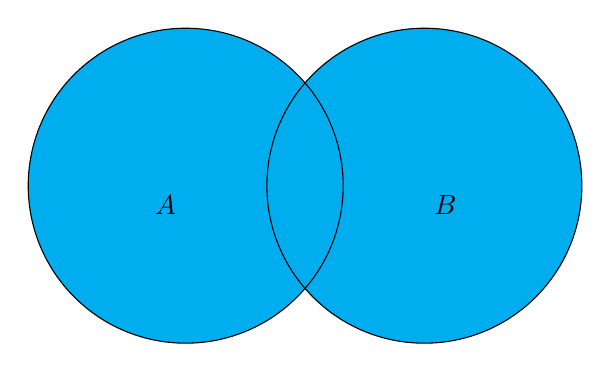
\begin{tikzpicture}
     % \begin{scope}
      %   \clip \secondcircle;
         \fill[cyan]  \thirdcircle;
         \fill[cyan] \secondcircle;
     % \end{scope}
      \draw \secondcircle node [text=black,below left] {$A$};
      \draw \thirdcircle node [text=black,below right] {$B$};
    \end{tikzpicture}
    \caption{Union $A\cup B$}
%\label{fig:my_label}
    \end{figure}
\end{center}

\end{frame}


\begin{frame}
\frametitle{Venn Diagram $A\cap B$}
\begin{center}
\begin{figure}
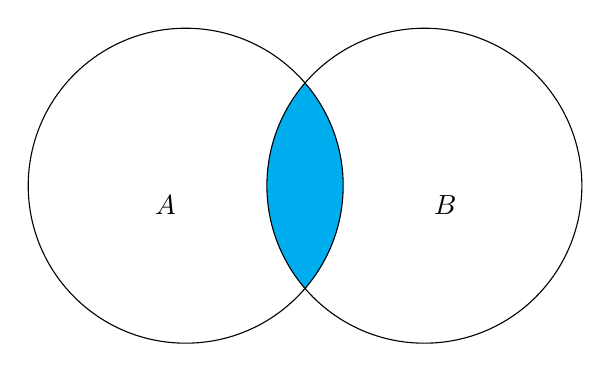
\begin{tikzpicture}
      \begin{scope}
         \clip \secondcircle;
         \fill[cyan] \thirdcircle;
      \end{scope}
      \draw \secondcircle node [text=black,below left] {$A$};
      \draw \thirdcircle node [text=black,below right] {$B$};
    \end{tikzpicture}
    \caption{Intersection $A\cap B$}
%\label{fig:my_label}
    \end{figure}
\end{center}

\end{frame}


\begin{frame}
\frametitle{Venn Diagram $A\setminus B$}
\begin{center}
\begin{figure}
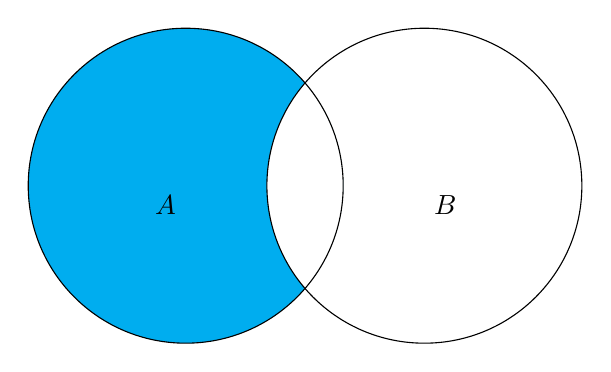
\begin{tikzpicture}
      \begin{scope}
         \clip \secondcircle;
         \fill[cyan] \secondcircle;
         \fill[white] \thirdcircle;
      \end{scope}
      \draw \secondcircle node [text=black,below left] {$A$};
      \draw \thirdcircle node [text=black,below right] {$B$};
    \end{tikzpicture}
    \caption{Set minus $A\setminus B$}
%\label{fig:my_label}
    \end{figure}
\end{center}

\end{frame}

\begin{frame}
\frametitle{Some Useful Properties}
\begin{itemize}
\item $\emptyset \subseteq A$
\bigskip
\item $A\cup \emptyset=A$ and $A \cap \emptyset=\emptyset$
 \bigskip

\item \textbf{De Morgan's laws}:
\[
\begin{aligned}
\overline{(A\cup B)}&=\overline{A}\cap \overline{B} \\ 
\overline{(A\cap B)}&=\overline{A}\cup \overline{B}\\
\overline{\overline{A}}&=A
\end{aligned}
\] 

\end{itemize}
\end{frame}

\begin{frame}
\frametitle{Set in Python}
\begin{center}
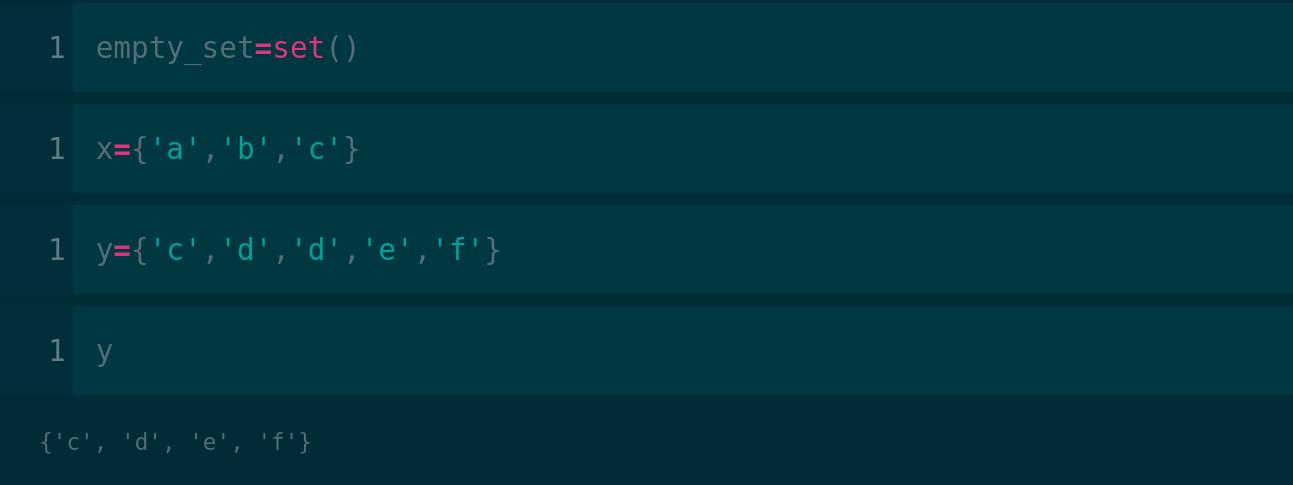
\includegraphics[scale=0.3]{set}
\end{center}
\end{frame}

\begin{frame}
\frametitle{Set in Python}
\begin{center}
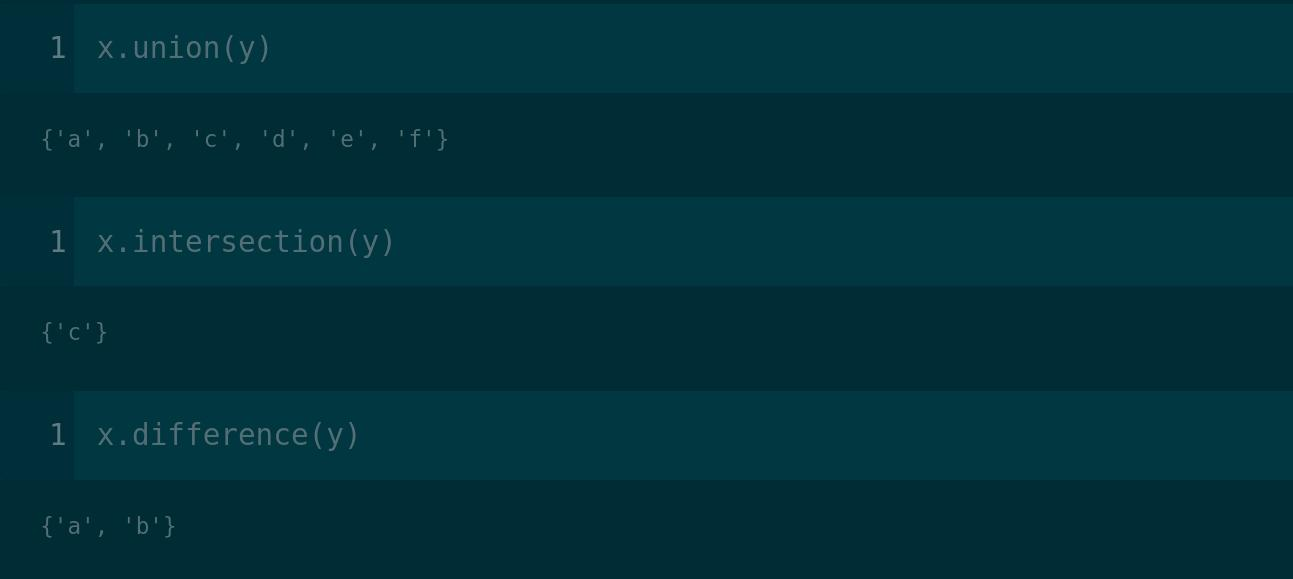
\includegraphics[scale=0.3]{union}
\end{center}
\end{frame}


\begin{frame}
\frametitle{Set in Python}
\begin{center}
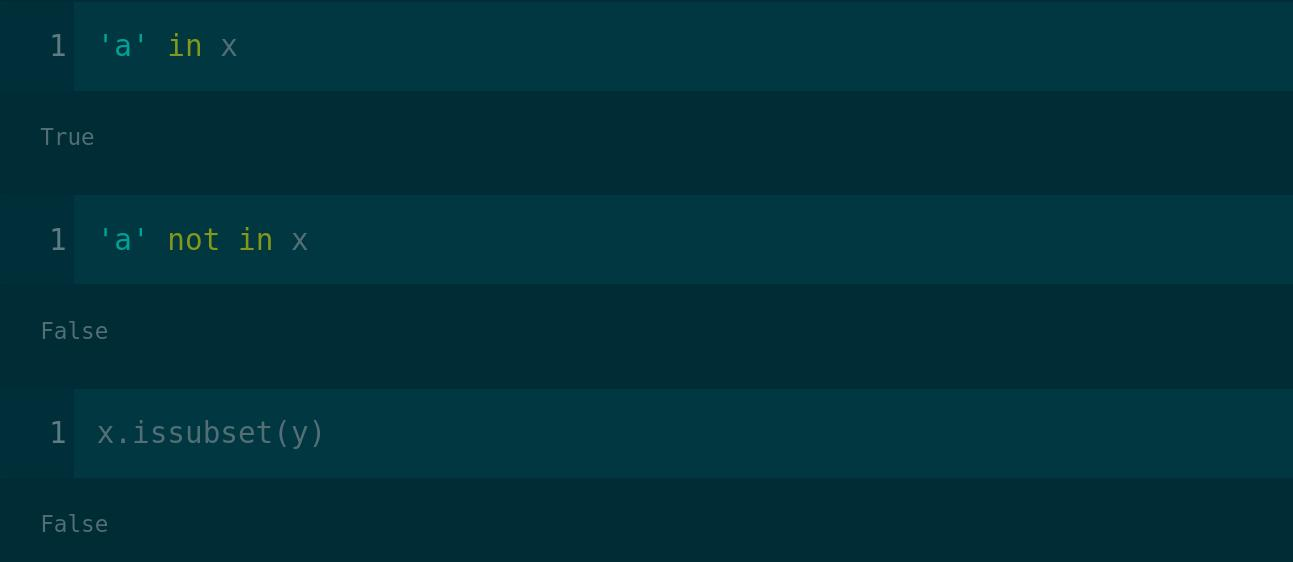
\includegraphics[scale=0.3]{member}
\end{center}
\end{frame}

\begin{frame}
\frametitle{Cartesian Product}
\begin{itemize}
\item The \textbf{Cartesian Product} of sets $A$ and $B$, denoted $A\times B$, 
is the set of all ordered pairs $(a,b)$ such that $a\in A$ and $b\in B$, i.e.,\pause
\[
A\times B=\{(a,b):a\in A\text{ and } b\in B\}
\] 
\pause
\item If $A=\{Joe, Philip\}$ and $B=\{Daniel, Peter, Joe\}$ then: \pause
\[
\begin{aligned}
A\times B = \{&(Joe, Daniel), (Joe, Peter), (Joe, Joe),\\
& (Philip, Daniel),(Philip, Peter), (Philip, Joe)\}
\end{aligned}
\]
\pause
\item \textcolor{red}{$A\times B \neq B\times A$}
\bigskip \pause
\item A \textbf{relation} between $A$ and $B$ is a subset of $A\times B$.

\end{itemize}
\end{frame}

\begin{frame}
\frametitle{Functions}
\begin{itemize}
\item A \textcolor{red}{\textbf{function}} is a relation between two sets such that each element of the first set is related to at most one element of the second set. \pause
\bigskip
\item Temperature of a cup of coffee is a function of time.
\bigskip
\item Stock price with respect to time.
\bigskip
\item Area of a circle with respect to its radius.
\end{itemize}
\end{frame}



\begin{frame}
\frametitle{Formal Definition}
\begin{itemize}
\item A function $f$ from set $A$ to set $B$, denoted $f:A\to B$, is a subset of $A\times B$ such that: \pause
\[
(a_1,b_1),(a_2,b_2)\in f \textbf{ and } a_1=a_2\Longrightarrow b_1=b_2
\]
\bigskip\pause
\item If $(a,b)\in f$ we write $f(a)=b$.
\bigskip \pause
\item So if $a_1=a_2$ then $f(a_1)=f(a_2)$.
\end{itemize}
\end{frame}

\begin{frame}
An vector is a mathematical object which has a \textbf{magnitude} and a \textbf{direction}:\pause
\begin{figure}
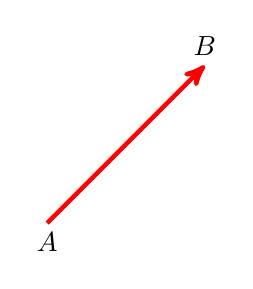
\begin{tikzpicture}
\draw[ultra thick,red] (0,0) -- (2,2);\pause
\node (0,0)[below] {$A$};\pause
\node at (2,2) [above] {$B$}; \pause
\end{tikzpicture}
\end{figure}
In this case we refer to this vector as $\overrightarrow{AB}$.
\end{frame}

\begin{frame}
We can add two vectors:\pause
\begin{figure}
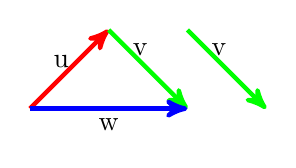
\begin{tikzpicture}
\node[above] at (0.4,0.4) {u};
\draw[ultra thick,red] (0,0) -- (1,1); \pause
\node[above] at (2.4,0.55) {v};
\draw[ultra thick, green] (2,1) -- (3,0); \pause
\node[above] at (1.4,0.55) {v};
\draw[ultra thick, green] (1,1) -- (2,0); \pause
\node[below] at (1,0) {w};
\draw[ultra thick, blue] (0,0) -- (2,0); 
\end{tikzpicture}
\end{figure}
\end{frame}

\begin{frame}
$-u$:\pause
\begin{figure}
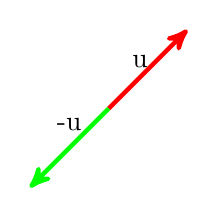
\begin{tikzpicture}
\node[above] at (0.4,0.4) {u};
\draw[ultra thick,red] (0,0) -- (1,1); \pause
\node[above] at (-0.5,-0.4) {-u};
\draw[ultra thick, green] (0,0) -- (-1,-1); 
\end{tikzpicture}
\end{figure}
\end{frame}

\begin{frame}
$v-u=v+(-u)=w$: \pause
\begin{figure}
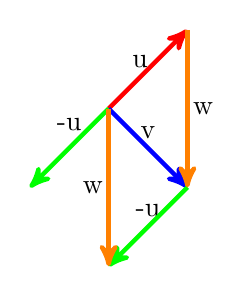
\begin{tikzpicture}
\node[above] at (0.4,0.4) {u};
\draw[ultra thick,red] (0,0) -- (1,1); \pause
\node[above] at (0.5,-0.5) {v};
\draw[ultra thick, blue] (0,0) -- (1,-1); \pause
\node[above] at (-0.5,-0.4) {-u};
\draw[ultra thick, green] (0,0) -- (-1,-1); \pause
\node[above] at (0.5,-1.5) {-u};
\draw[ultra thick, green] (1,-1) -- (0,-2);\pause
\node[above] at (-0.2,-1.2) {w};
\draw[ultra thick, orange] (0,0) -- (0,-2);\pause
\node[above] at (1.2,-0.2) {w};
\draw[ultra thick, orange] (1,1) -- (1,-1);
\end{tikzpicture}
\end{figure}
\end{frame}

\begin{frame}
We can consider a reference and put the starting point of all vectors in this reference point, call it $\mathbf{O}$. So in two dimentions we will write a vector as:
\[
\begin{bmatrix}
x_1\\
x_2
\end{bmatrix}
\]
\end{frame}

\begin{frame}
\begin{figure}
\begin{tikzpicture}
\tkzInit[xmax=7,ymax=7,xmin=-7,ymin=-1]
   \tkzGrid
   \tkzAxeXY
   \draw[thick, red] (0,0) -- (3,5);
   \node[] at (3.3,5) {$\begin{bmatrix}
   3\\
    5
   \end{bmatrix}$};\pause
   \draw[thick, green] (0,0) -- (4,2);
   \node[] at (4.3,2) {$\begin{bmatrix}
   4\\
    2
   \end{bmatrix}$};\pause
   \draw[thick, blue] (0,0) -- (7,7);
   \node[] at (7.3,7) {$\begin{bmatrix}
   7\\
   7
   \end{bmatrix}$};\pause
   \draw[thick, green] (3,5) -- (7,7);
   \node[] at (3.3,5) {$\begin{bmatrix}
   3\\
    5
   \end{bmatrix}$};\pause
   \draw[thick, orange] (0,0) -- (-1,3);
   \node[] at (-1.4,3) {$\begin{bmatrix}
   -1\\
    3
   \end{bmatrix}$};\pause
   \draw[thick, orange] (4,2) -- (3,5);
   \node[] at (-1.4,3) {$\begin{bmatrix}
   -1\\
    3
   \end{bmatrix}$};
   
  % \draw[ thick,latex-latex] (-1,4) -- (4,-6) node[anchor=south west] {$a$}; % two points for drawing 2x+y=2
  \end{tikzpicture}
\end{figure}
\end{frame}

\begin{frame}
\frametitle{Algebra of Vectors}
\[
\mathbf{O}=\begin{bmatrix}
0\\
0
\end{bmatrix}
\]\pause
\[
\begin{bmatrix}
x_1\\
x_2
\end{bmatrix}+
\begin{bmatrix}
x_1'\\
x_2'
\end{bmatrix}=\begin{bmatrix}
x_1+x_1'\\
x_2+x_2'
\end{bmatrix}
\]\pause
\[
\begin{bmatrix}
x_1\\
x_2
\end{bmatrix}-
\begin{bmatrix}
x_1'\\
x_2'
\end{bmatrix}=\begin{bmatrix}
x_1-x_1'\\
x_2-x_2'
\end{bmatrix}
\]\pause
\[
c\begin{bmatrix}
x_1\\
x_2
\end{bmatrix}=\begin{bmatrix}
cx_1\\
cx_2
\end{bmatrix}
\]
\end{frame}

\begin{frame}
\frametitle{n-dimensional vectors}
The set of all $n$-dimensional vectors,\pause
\[
\begin{bmatrix}
x_1\\
\vdots\\
x_n
\end{bmatrix}
\]\pause
is denoted by $\Re^n$.
\end{frame}

\begin{frame}
\frametitle{Euclidean Length of Vectors}
The Euclidean length of a vecor,\pause
\[u=
\begin{bmatrix}
x_1\\
\vdots\\
x_n
\end{bmatrix}
\]\pause
is denoted by $\|\mathbf{u}\|$ and is a real number that represent the length of $u$ and is calculated by,\pause
\[
\|\mathbf{u}\|=\sqrt{x_1^2+\dots +x_n^2}
\]
\end{frame}

\begin{frame}
\frametitle{Inner Product}
The \textbf{inner product} of two vectors $\mathbf{u}$ and $\mathbf{v}$ is a real number defined by the following formula,\pause
\[
\mathbf{u}\cdot \mathbf{v}=\|\mathbf{u}\|\|\mathbf{v}\|cos(\theta)
\]\pause
where $\theta$ is the angel between $\mathbf{u}$ and $\mathbf{v}$.
\begin{figure}
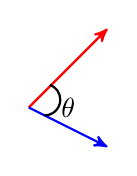
\begin{tikzpicture}
\draw[thick, red] (0,0) -- (1,1);
\draw[thick, blue] (0,0) -- (1,-0.5);
\draw[thick, -] (0.2,-0.1) arc (-90:70:0.2);
\node[] at (0.5,0) {$\theta$};
\end{tikzpicture}
\end{figure}
\end{frame}

\begin{frame}
If,\pause
\[\mathbf{u}=
\begin{bmatrix}
x_1\\
\vdots\\
x_n
\end{bmatrix}\,\, ,
\mathbf{v}=
\begin{bmatrix}
y_1\\
\vdots\\
y_n
\end{bmatrix}
\]\pause
then \pause
\[
\mathbf{u}\cdot \mathbf{v}=x_1y_1+\dots+x_ny_n
\]
\end{frame}

\begin{frame}
If $\mathbf{u}\cdot \mathbf{v}=0$ then $\mathbf{u}$ is perpendicular with $\mathbf{v}$.\pause
\begin{figure}
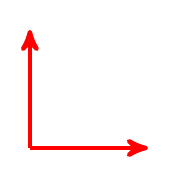
\begin{tikzpicture}
\draw[ultra thick,red] (0,0) -- (0,1.5);
\draw[ultra thick,red] (0,0) -- (1.5,0);
\end{tikzpicture}
\end{figure}
\end{frame}
%
%\begin{frame}
%Let $\|\mathbf{u}\|=1$ then $\mathbf{u}\cdot \mathbf{v}$ is the length of projection of $\mathbf{v}$ in the direction of $\mathbf{u}$,\pause
%\begin{figure}
%\begin{tikzpicture}
%\draw[ultra thick, red] (0,0) -- (2,2);\pause
%\draw[ultra thick, green] (0,0) -- (1,0);\pause
%\draw[thick] (2,2) -- (2,0);\pause
%\draw[ultra thick,blue] (0,0) -- (2,0);
%\end{tikzpicture}
%\end{figure}
%\end{frame}


\begin{frame}
Let $\|\mathbf{u}\|=1$ then $\mathbf{u}\cdot \mathbf{v}$ is the length of projection of $\mathbf{v}$ in the direction of $\mathbf{u}$,\pause
\begin{figure}
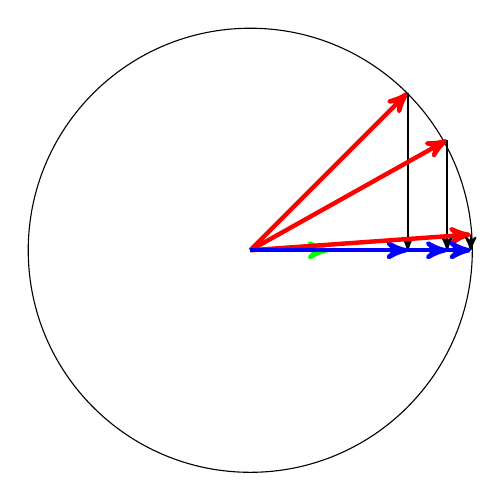
\begin{tikzpicture}
\draw[ultra thick, red] (0,0) -- (2,2);\pause
\draw[ultra thick, green] (0,0) -- (1,0);\pause
\draw[thick] (2,2) -- (2,0);\pause
\draw[ultra thick,blue] (0,0) -- (2,0);\pause

\draw[] (0,0) circle (2.82);\pause

\draw[ultra thick, red] (0,0) -- (2.5,1.4);\pause
\draw[thick] (2.5,1.4) -- (2.5,0);\pause
\draw[ultra thick,blue] (0,0) -- (2.5,0);\pause

\draw[ultra thick, red] (0,0) -- (2.8,0.2);\pause
\draw[thick] (2.8,0.2) -- (2.8,0);\pause
\draw[ultra thick,blue] (0,0) -- (2.8,0);
\end{tikzpicture}
\end{figure}
\end{frame}

\begin{frame}
So, $\mathbf{u}\cdot \mathbf{v}$ is maximum if $\mathbf{v}$ is in the same direction as $\mathbf{u}$.\pause
\begin{figure}
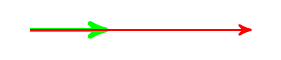
\begin{tikzpicture}
\draw[ultra thick, green] (0,0) -- (1,0);
\draw[thick, red] (0,0) -- (2.82,0);
\end{tikzpicture}
\end{figure}
\end{frame}

\begin{frame}
\frametitle{Vectors in Python}
\begin{center}
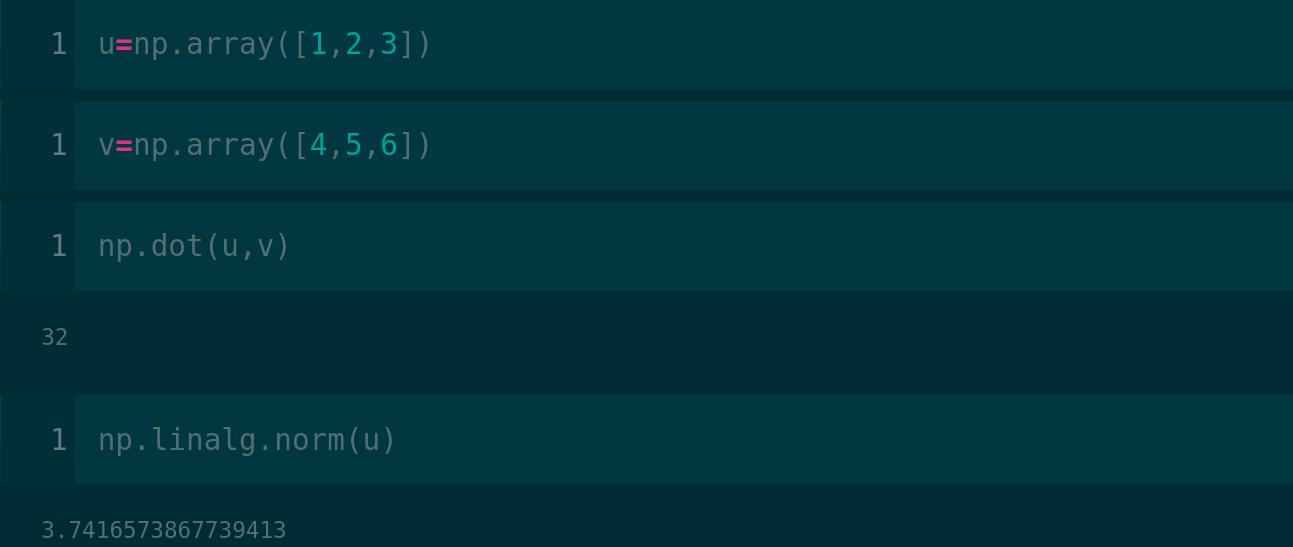
\includegraphics[scale=0.3]{vec}
\end{center}
\end{frame}

\begin{frame}
\frametitle{Vectors in Python}
\begin{center}
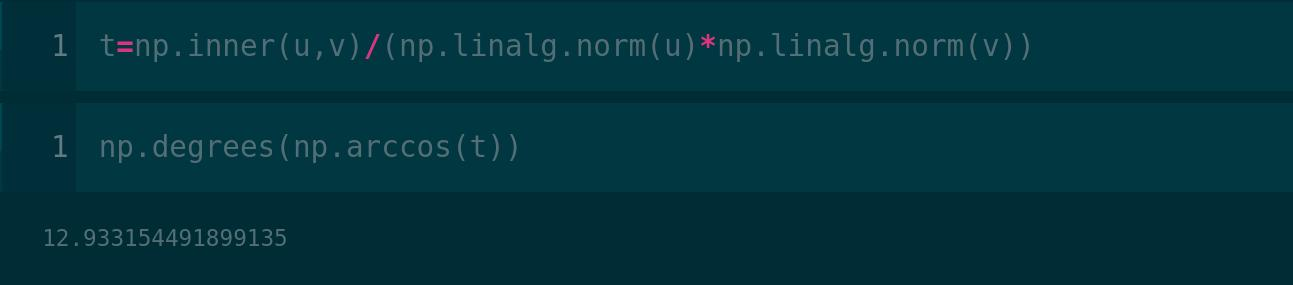
\includegraphics[scale=0.3]{vec2}
\end{center}
\end{frame}

\begin{frame}
\frametitle{Matrices}
Matrix is a two-dimensional array-like data structure that represents a common quantity of two categories. For example, if you want to represent the number of students by gender in three different class of Math, CS, and Physic then you should use matrix representation as follow;
\[
\begin{array}{c c} &
\begin{array}{c c c} \textcolor{red}{Math} & \textcolor{red}{CS} & \textcolor{red}{Physic} \\
\end{array}
\\
\begin{array}{c c c}
\textcolor{blue}{Men} \\
\textcolor{blue}{Women}
\end{array}
&
\left[
\begin{array}{c c c}
23 & 37 & 18 \\
28 & 14 & 16 
\end{array}
\right]
\end{array}
\]
\end{frame}

\begin{frame}
If a matrix has $m$ rows and $n$ columns then we say the \textbf{order} of the matrix is $m\times n$. So an $n$-dimensional vector is a special case of a matrix of order $n\times 1$.  
\end{frame}



\begin{frame}
A \textbf{square matrix} is a matrix that have the same number of rows and columns, i.e., $m=n$.\\ \pause
An \textbf{identity matrix} is a square matrix with $1$ in the main diagonal and $0$ elsewhere. We denote the identity matrix of order $n$ by $\mathbf{I}_n$. \pause 
\[
\mathbf{I}_n=
\begin{bmatrix}
1 & 0 & \dots & 0\\
0 & 1 & \dots & 0\\
\vdots & \vdots & \ddots & \vdots\\
0 & 0 & \dots & 1
\end{bmatrix}
\]
\end{frame}


\begin{frame}
The \textbf{zero matrix} is a matrix such that every entries is $0$. We denote the zero matrix of order $m\times n$ by $\mathbf{O}_{m\times n}$. \pause 
\[
\mathbf{O}_{m\times n}=
\begin{bmatrix}
0 & 0 & \dots & 0\\
0 & 0 & \dots & 0\\
\vdots & \vdots & \ddots & \vdots\\
0 & 0 & \dots & 0
\end{bmatrix}
\]
\end{frame}

\begin{frame}
Transpose of an $m\times n$ matrix is an $n\times m$ matrix. The transpose of the matrix $\mathbf{A}$ is denoted by $\mathbf{A}^T$.\pause
\[\mathbf{A}=
\begin{bmatrix}
1 & 2 & 3\\
4 & 5 & 6
\end{bmatrix}
\]\pause
\[\mathbf{A}^T=
\begin{bmatrix}
1 & 4\\
2 & 5\\
3 & 6
\end{bmatrix}
\]
\end{frame}

\begin{frame}
We could add or subtract two matrices of the same order by adding or subtracting the corresponding entries together.\pause
\[
\begin{bmatrix}
1 & 2 & 3\\
4 & 5 & 6
\end{bmatrix}
+\pause
\begin{bmatrix}
3 & 0 & 1\\
2 & -1 & 2
\end{bmatrix}
=\pause
\begin{bmatrix}
1+3 & 2+0 & 3+1\\
4+2 & 5+(-1) & 6+2
\end{bmatrix}
\]
\end{frame}

\begin{frame}
If $\mathbf{A}_{1\times n}$ and $\mathbf{B}_{n\times 1}$ then we could define $\mathbf{AB}$ as follow,\pause
\[
\begin{bmatrix}
a_1 & \dots & a_n
\end{bmatrix}
\begin{bmatrix}
b_1\\
\vdots\\
b_n
\end{bmatrix}=
a_1b_1+\dots + a_nb_n
\]
So if $\mathbf{u}$ and $\mathbf{v}$ are $n$-dimensional vectors then, \pause
\[
\mathbf{u}\cdot \mathbf{v}=\mathbf{u}^T\mathbf{v}
\]
\end{frame}

\begin{frame}
If $\mathbf{A}_{m\times n}$ and $\mathbf{B}_{n\times k}$ then we could define $\mathbf{AB}$ as the following $m\times k$ matrix,
\[
\begin{bmatrix}
a_{11} & \dots & a_{1n}\\
\vdots & \ddots & \vdots\\
a_{m1} & \dots & a_{mn}
\end{bmatrix}
\begin{bmatrix}
b_{11} & \dots & b_{1k}\\
\vdots & \ddots & \vdots\\
b_{n1} & \dots & b_{nk}
\end{bmatrix}=
\begin{bmatrix}
 & \vdots & \\
\dots &
\begin{bmatrix}
a_{i1} & \dots & a_{in}
\end{bmatrix}
\begin{bmatrix}
b_{1j}\\
\vdots\\
b_{nj}
\end{bmatrix} & \dots & \\
 & \vdots & \\
\end{bmatrix}
\]
\end{frame}

\begin{frame}
\frametitle{Inverse of Matrix}
If for the square matrix $\mathbf{A}$ there exists another square matrix $\mathbf{B}$ such that,
\[
\mathbf{AB}=\mathbf{BA}=\mathbf{I}
\]
then we say $\mathbf{A}$ is invertible and its inverse is $\mathbf{B}$. We denote $\mathbf{B}$ by $\mathbf{A}^{-1}$.
\end{frame}

\begin{frame}
If $\mathbf{A}$ is invertible then the system of equations,
\[
\mathbf{Ax}=\mathbf{b}
\]
has a unique solution, i.e.,
\[
\mathbf{x}=\mathbf{A}^{-1}\mathbf{b}
\]
\end{frame}

\begin{frame}
\[
\begin{aligned}
& \mathbf{IA}=\mathbf{AI}=\mathbf{A}\\ \pause
& (\mathbf{A}+\mathbf{B})^T=\mathbf{A}^T+\mathbf{B}^T \\ \pause
& (\mathbf{AB})^T=\mathbf{B}^T\mathbf{A}^T \pause
\end{aligned}
\]
A symmetric matrix is a square matrix such that $\mathbf{A}^T=\mathbf{A}$.
\end{frame}

\begin{frame}
\frametitle{Tensors}
\textbf{Tensors} are multi-dimensional array with a uniform type. 
A tensor of order $m\times n\times k$ (or shape $(m,n,k)$) is actually $m$ matrices of order $n\times k$. 

\end{frame}

\begin{frame}
\[
\begin{bmatrix}
\begin{bmatrix}
1 & 2 & 3\\
4 & 5 & 6
\end{bmatrix}\\ 
\begin{bmatrix}
7 & 8 & 9\\
10 & 11 & 12
\end{bmatrix}\\ 
\begin{bmatrix}
13 & 14 & 15\\
16 & 17 & 18
\end{bmatrix}\\
\begin{bmatrix}
19 & 20 & 21\\
22 & 23 & 24
\end{bmatrix}
\end{bmatrix}
\]
is a tensor of order $4\times 2 \times 3$
\end{frame}

\begin{frame}
$3\times 2 \times 3$ tensor.
\begin{center}
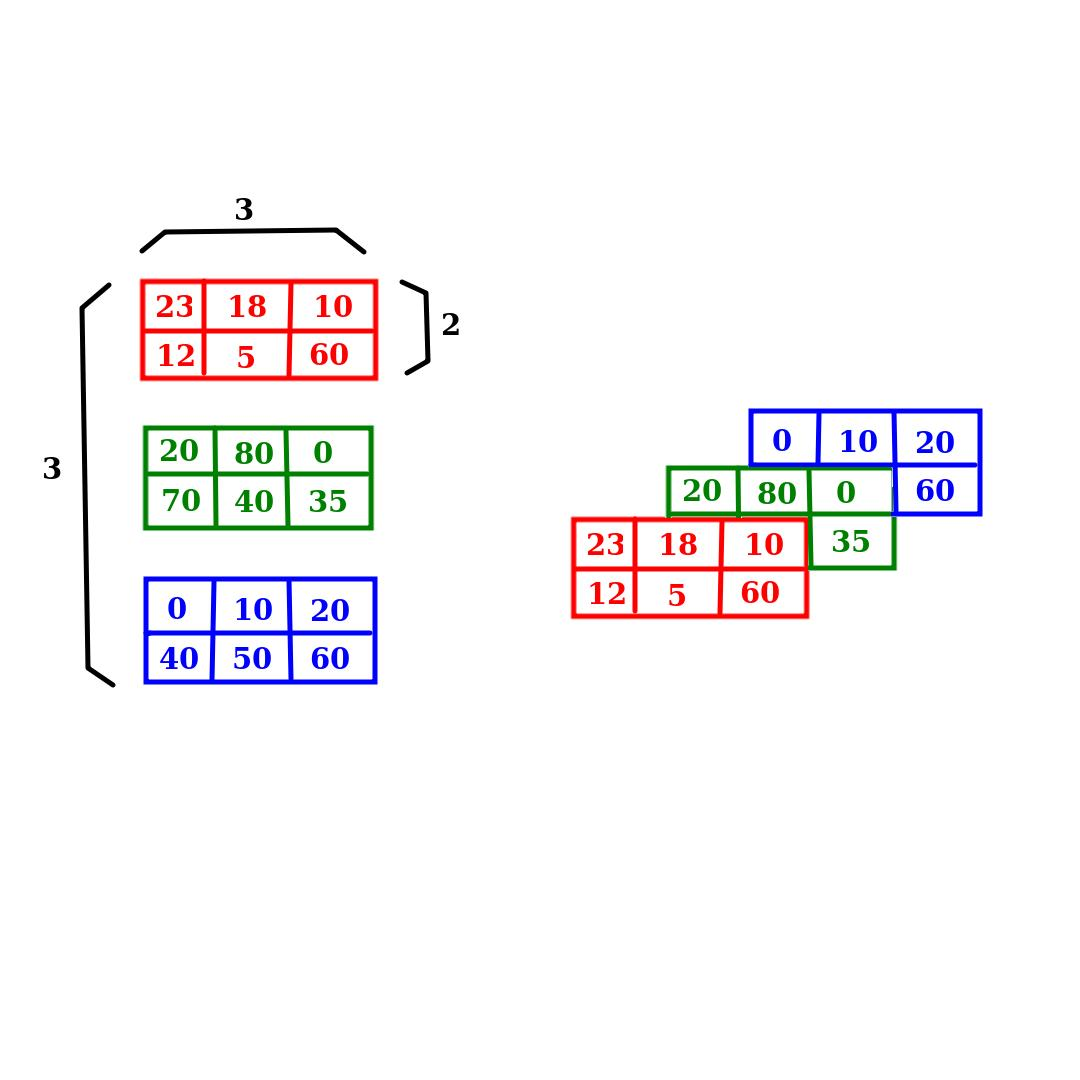
\includegraphics[scale=0.3]{tensor}
\end{center}

\end{frame}

\begin{frame}
\frametitle{Kronecker(Tensor) Product}
The \textbf{Kronecker product} of matrices $\mathbf{A}_{m\times n}$ and $\mathbf{B}_{k\times l}$ is a matrix of order $mk\times nl$ and define as follow,
\[
\mathbf{A}\otimes \mathbf{B}=
\begin{bmatrix}
a_{11}\mathbf{B} & \dots & a_{1n}\mathbf{B}\\
\vdots & \ddots & \vdots\\
a_{m1}\mathbf{B} & \dots & a_{mn}\mathbf{B}
\end{bmatrix}
\]
\end{frame}

\begin{frame}
\[
\begin{aligned}
\begin{bmatrix}
x_1 & x_2
\end{bmatrix} \otimes
\begin{bmatrix}
1 & 0\\
0 & 1
\end{bmatrix}&=
\begin{bmatrix}
x_1 \mathbf{I} & x_2\mathbf{I}
\end{bmatrix}\\
&=
\begin{bmatrix}
x_1 & 0 & x_2 & 0\\
0 & x_1 & 0 & x_2 
\end{bmatrix}\\
\end{aligned}
\]
\end{frame}

\begin{frame}
\frametitle{Eigenvalue}
Let $\mathbf{A}$ be an square $n\times n$ matrix. If there exists $n$-dimensional vector $\mathbf{v}$ and a real number $\lambda$ such that,
\[
\mathbf{Av}=\lambda\mathbf{v}
\]
then we say $\mathbf{v}$ is an eigenvector and the corresponding eigenvalue is $\lambda$.
\end{frame}

\begin{frame}
To obtain the eigenvalues of a matrix you need to find the roots of the following polynomal equation of order $n$,\pause
\[
det(\lambda \mathbf{I}-\mathbf{A})=0
\] \pause
eigenvalue could be complex number, i.e., a matrix may don't have any real valued eigenvalue but \pause all eigenvalues of a symmetric matrix are real numbers.\end{frame}

\begin{frame}
\frametitle{Rotation Matrix}
\[
\mathbf{R}_{\theta}=
\begin{bmatrix}
cos(\theta) & -sin(\theta)\\
sin(\theta) & cos(\theta)
\end{bmatrix}
\]\pause
\begin{figure}
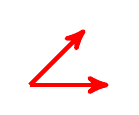
\begin{tikzpicture}
\draw[ultra thick, red] (0,0) -- (1,0);\pause
\draw[ultra thick, red] (0,0) -- (0.7,0.7);
\end{tikzpicture}
\end{figure}
\end{frame}

\begin{frame}
$\mathbf{R}_{\frac{\pi}{2}}$ has no eigenvalue but $\mathbf{R}_{\frac{\pi}{2}}^2$ has $-1$ as the only real eigenvalue.
\begin{figure}
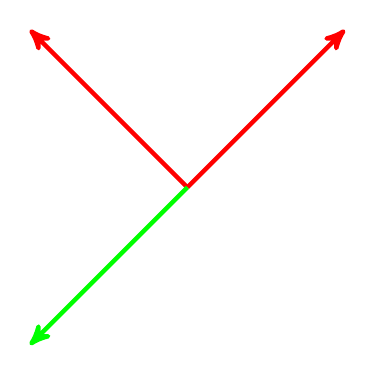
\begin{tikzpicture}
\draw[ultra thick, red] (0,0) -- (2,2);\pause
\draw[ultra thick, red] (0,0) -- (-2,2);\pause
\draw[ultra thick, green] (0,0) -- (-2,-2);
\end{tikzpicture}
\end{figure}
\end{frame}

\begin{frame}
\frametitle{Matrices in Python}
\begin{center}
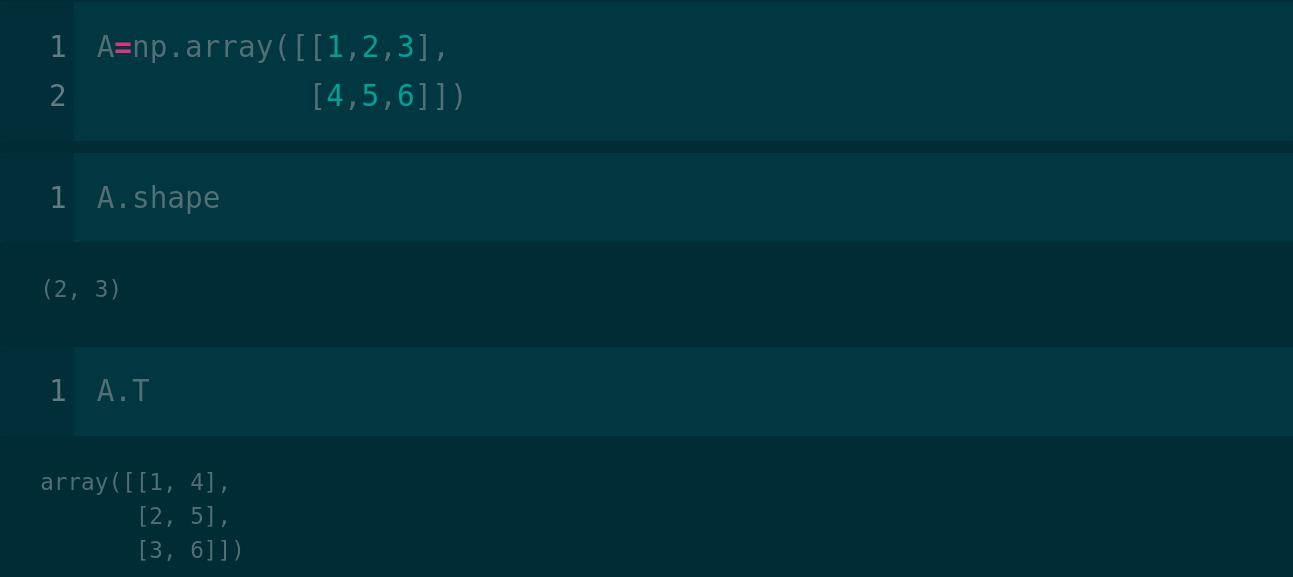
\includegraphics[scale=0.3]{mat}
\end{center}
\end{frame}

\begin{frame}
\frametitle{Matrices in Python}
\begin{center}
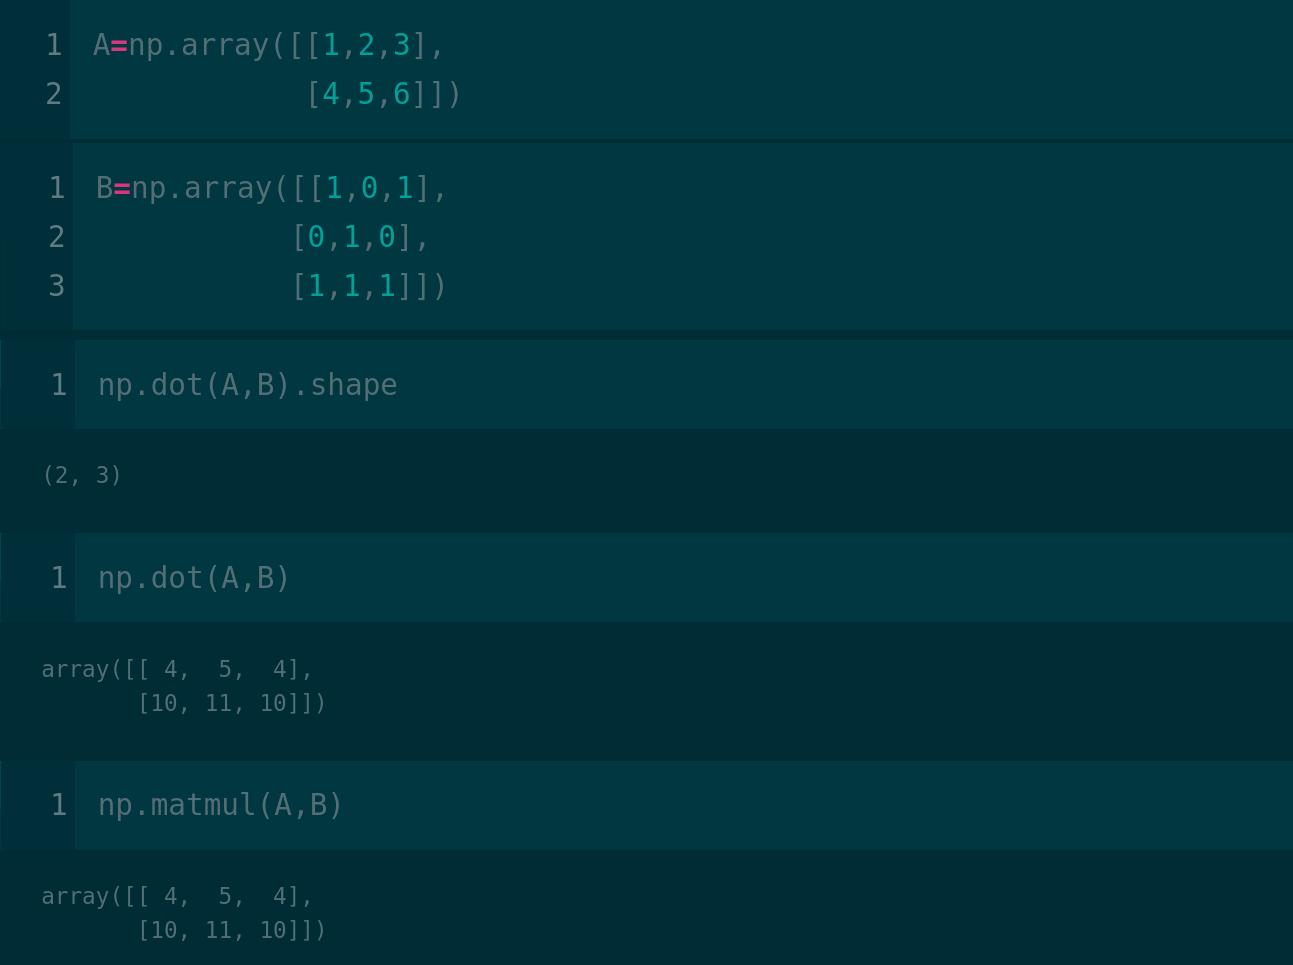
\includegraphics[scale=0.3]{mat2}
\end{center}
\end{frame}


\begin{frame}
\frametitle{Matrices in Python}
\begin{center}
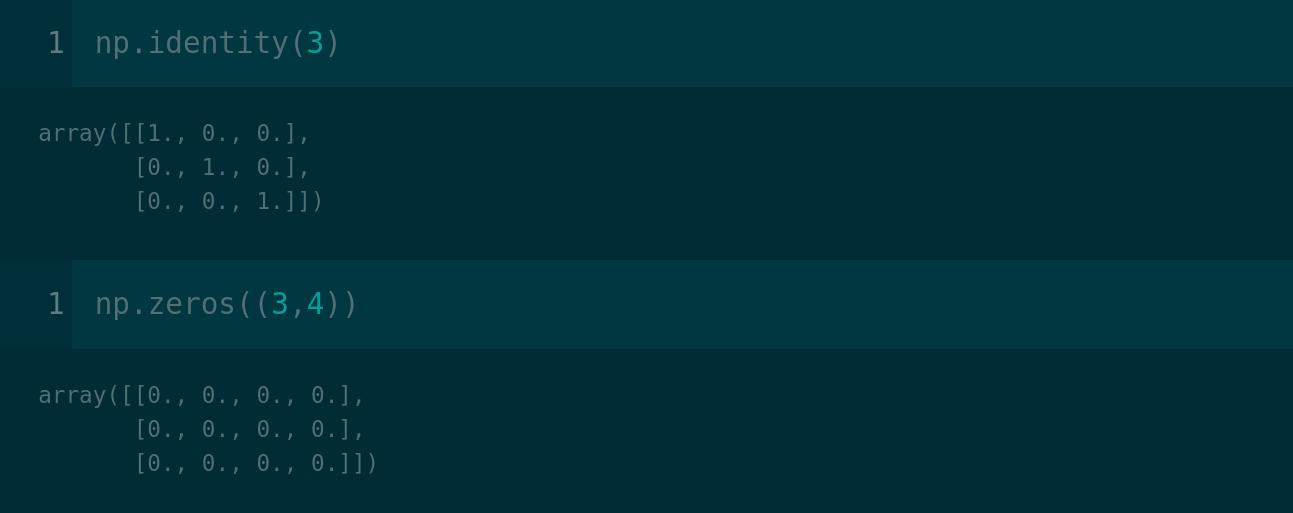
\includegraphics[scale=0.3]{mat3}
\end{center}
\end{frame}

\begin{frame}
\frametitle{Matrices in Python}
\begin{center}
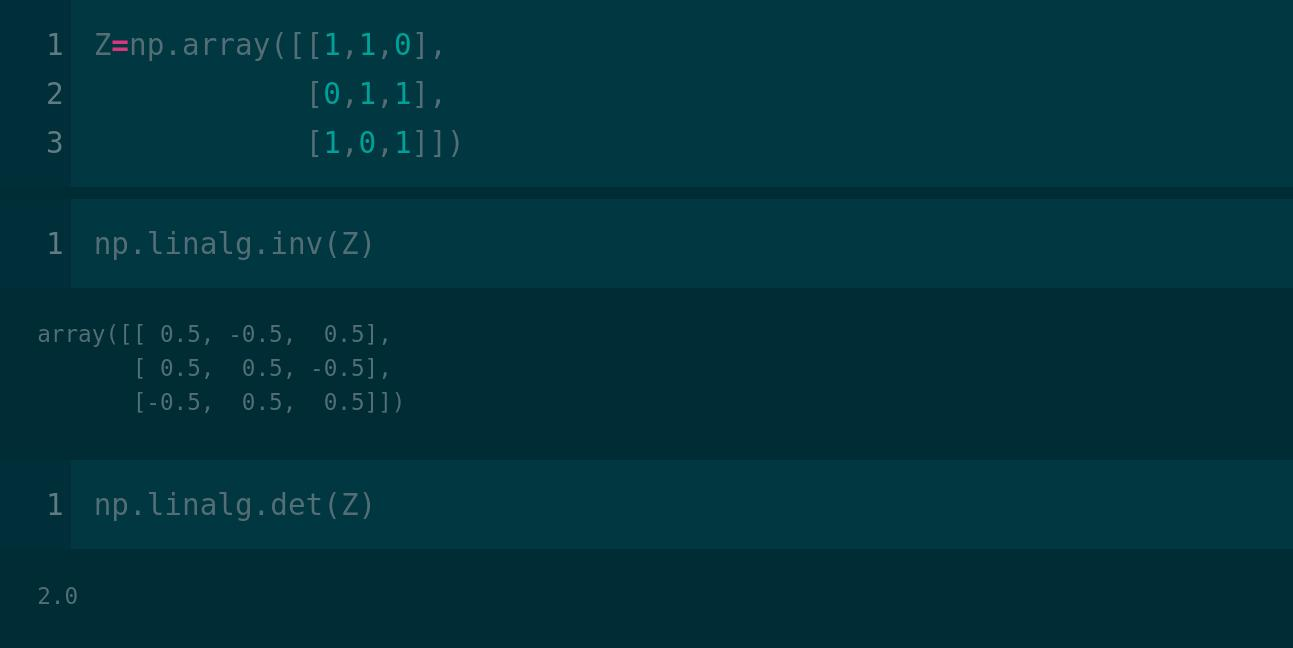
\includegraphics[scale=0.3]{mat4}
\end{center}
\end{frame}

\begin{frame}
\frametitle{Matrices in Python}
\begin{center}
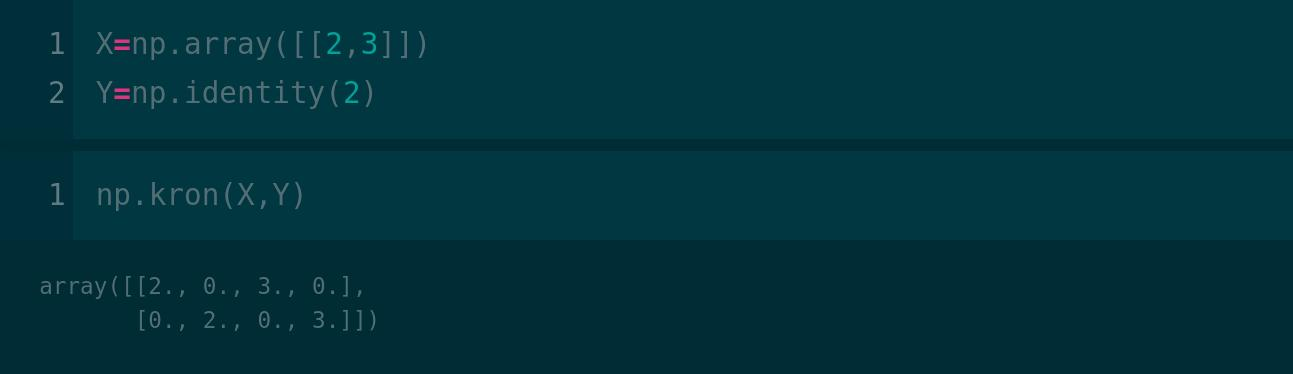
\includegraphics[scale=0.3]{mat5}
\end{center}
\end{frame}

\begin{frame}
\frametitle{Matrices in Python}
\begin{center}
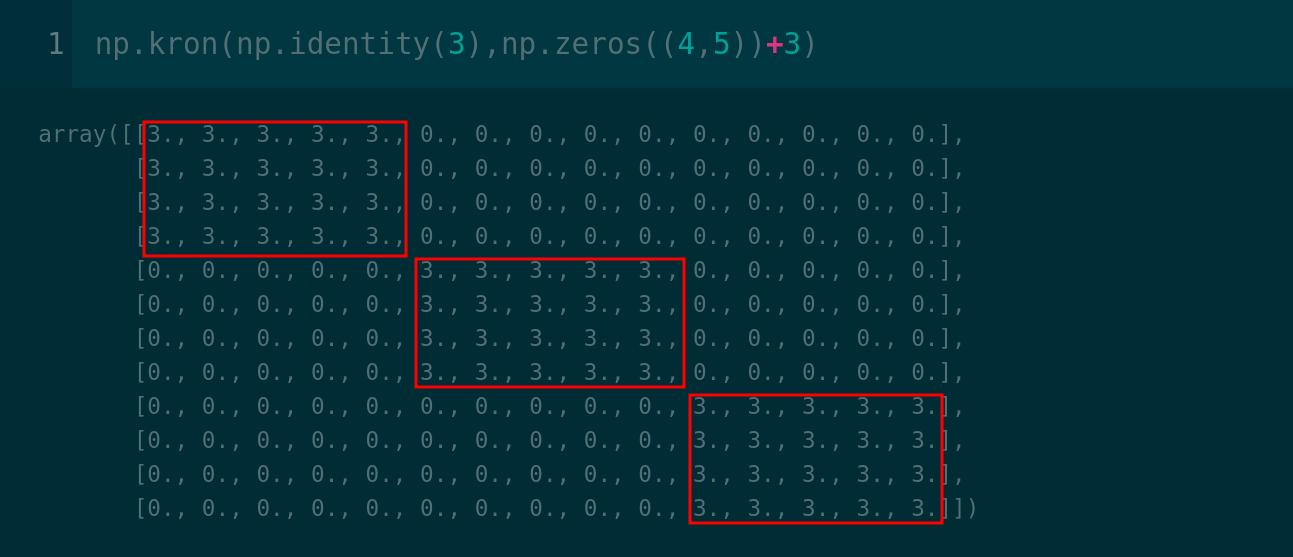
\includegraphics[scale=0.3]{mat6}
\end{center}
\end{frame}

\begin{frame}
\frametitle{Matrices in Python}
\begin{center}
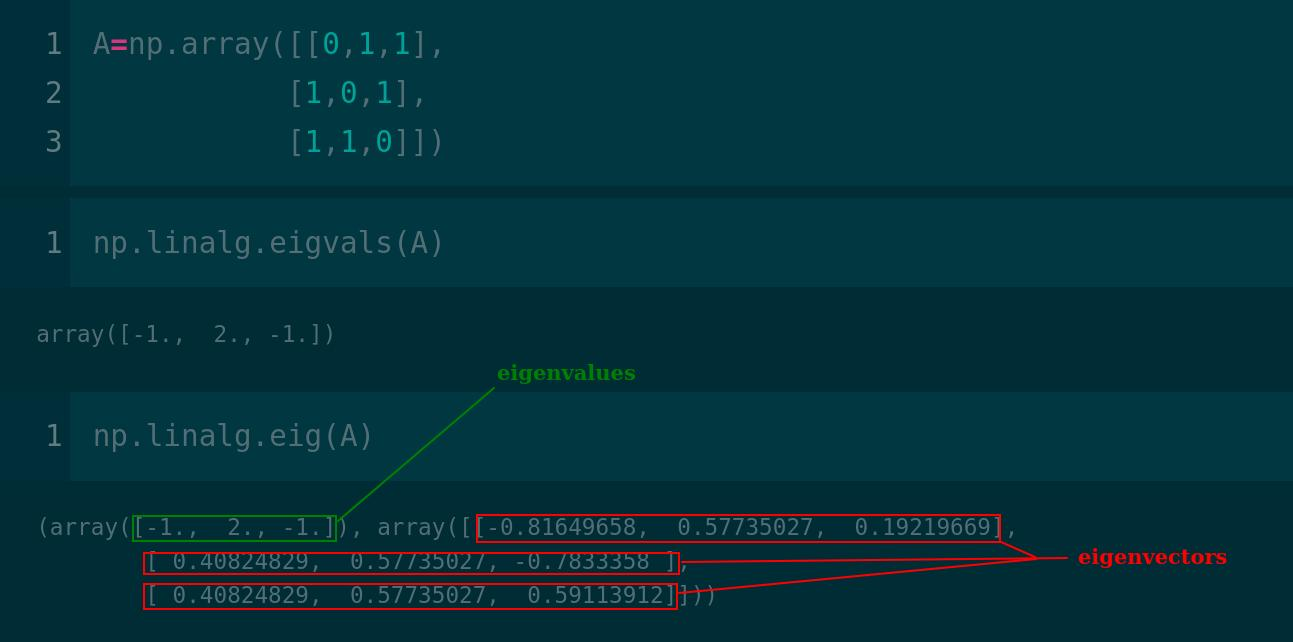
\includegraphics[scale=0.3]{mat7}
\end{center}
\end{frame}


\begin{frame}{}
  \centering \Huge
  \emph{Thank You}
\end{frame}

\end{document}

